% TEMPLATE FROM:
% NAME:		swift_scijust_template.tex
% Modified on 2/17/16 by Corey Mutnik

\documentclass[letterpaper,11pt]{article}
%\documentclass[letterpaper,11pt,twocolumn]{article

\usepackage{graphics,graphicx}
%\usepackage{psfig}
\usepackage{times}
\usepackage{float}	% allows use of 'H' command
%\usepackage[demo]{graphicx}
%\usepackage{caption}
\usepackage{subcaption}



%%%%%%%%%%%%%%%%%%%%%%%%%%%%%%%%%%%%%%%%%%%%%%%%%
%%%%% Page dimensions                       %%%%%
%%%%% DO NOT CHANGE THE FOLLOWING 9 LINES!  %%%%%
%%%%%%%%%%%%%%%%%%%%%%%%%%%%%%%%%%%%%%%%%%%%%%%%%

\setlength{\textwidth}{7in} 
\setlength{\textheight}{9.5in}
\setlength{\topmargin}{-0.2in} 
\setlength{\oddsidemargin}{-0.2in}
\setlength{\evensidemargin}{-0.2in} 
\setlength{\headheight}{0in}
\setlength{\headsep}{0in} 
\setlength{\hoffset}{0in}
\setlength{\voffset}{0in}


%%%%%%%%%%%%%%%%%%%%%%%%%%%%%%%%%%
%%%%% Section heading format %%%%%
%%%%%%%%%%%%%%%%%%%%%%%%%%%%%%%%%%

\makeatletter
\renewcommand{\section}{\@startsection%
{section}{1}{0mm}{-\baselineskip}%
{0.5\baselineskip}{\normalfont\Large\bfseries}}%
\makeatother



% DEFINE BOX ENVIRONMENT %%%%%%%%%%%%%%%%%%%%%%%%%%%%%%%%%%%%%%%%%%%%%%%%%%%%%%%%%%%%%%%%%%%%%%%%%%%%%%
%%%%%%%%%%%%%%%%%%%%%%%%%%%%%%%%%%%%%%%%%%%%%%%%%%%%%%%%%%%%%%%%%%%%%%%%%%%%%%%%%%%%%%%%%%%%%%%%%%%%%%%
\newsavebox\FrameBox
\newenvironment{Frame}{%
  \noindent\setbox\FrameBox\hbox\bgroup\minipage{1.01\textwidth}\parskip\baselineskip\ignorespaces
}{%
  \endminipage\egroup\fbox{\box\FrameBox}\par
}
%%%%%%%%%%%%%%%%%%%%%%%%%%%%%%%%%%%%%%%%%%%%%%%%%%%%%%%%%%%%%%%%%%%%%%%%%%%%%%%%%%%%%%%%%%%%%%%%%%%%%%%
%%%%%%%%%%%%%%%%%%%%%%%%%%%%%%%%%%%%%%%%%%%%%%%%%%%%%%%%%%%%%%%%%%%%%%%%%%%%%%%%%%%%%%%%%%%%%%%%%%%%%%%



\begin{document}
\pagestyle{plain}
\pagenumbering{arabic}

\begin{center} 
\bfseries\uppercase{\Large{University of Hawaii $\bullet$ Institute for Astronomy} \\ 
\large{Research Proposal -- Observing Time Request}}
\end{center}
\vspace{-0.3cm}


\iffalse
	% box around names, emails, and institution
	\noindent\fbox{\linespread{1.5}
		\parbox{\textwidth}{\bf{
				Names: {Daichi Hiramatsu} \& {Corey Mutnik} \\
				E-mails: dhiramat@hawaii.edu \& cmutnik@hawaii.edu\\
				Institution/Dept: UH
			}
		}
	} 
	~\\ %this is here to make gap between boxes
	% box around program titles
	\noindent\fbox{\linespread{1.5}
		\parbox{\textwidth}{\bf{
				Program Title\\
				A. Measuring the Milky Way\\
				B.\\
				C.
			}
		}
	} 
\fi


\noindent\fbox{\linespread{2}
  \parbox{\textwidth}{\bf{
	\begin{minipage}{0.5\textwidth}
		\begin{flushleft}
	    	\subsection*{Author$^{*}$~:~Daichi~Hiramatsu}
	    	%\subsection*{Author$_{1}$~:~Daichi~Hiramatsu\\E-mail$_{1}$~:~dhiramat@hawaii.edu}
		\end{flushleft}
	\end{minipage}
  \hfill
	\begin{minipage}{0.5\textwidth}
		\begin{flushright}
	    	\textbf{\large Author$^{\dagger}$~:~Corey Mutnik~~}\\[1.5cm]
		\end{flushright}
	\end{minipage}
	\begin{minipage}{0.5\textwidth}
		\begin{flushleft}
			\subsection*{E-mail$^{*}$~:~dhiramat@hawaii.edu}
		\end{flushleft}
	\end{minipage}
  \hfill
	\begin{minipage}{0.5\textwidth}
		\begin{flushright}
	    	\textbf{\large E-mail$^{\dagger}$~:~cmutnik@hawaii.edu~~}\\[1.5cm]
		\end{flushright}
	\end{minipage}

	\subsection*{Institution/Dept$^{*,\dagger}$~:~UH}
  }
 }
}

~\\~\\ % for gap between frames

\noindent\fbox{\linespread{1.5}
	\parbox{\textwidth}{\bf{
			Program Title\\
			A. Measuring the Milky Way\\
			B.\\
			C.
		}
	}
} 

~\\~\\ % for gap between frames

\begin{Frame}
\noindent {\bf \\Abstract}
\smallskip%\\

Using various data reduction techniques, we will measure the size, shape, and age of the Milky Way galaxy's spiral arms.
% can report variable stars to AAVSO:
% https://www.aavso.org/how-report-new-variable-star-discoveries

\end{Frame}
~\\
\section*{TELESCOPE TIME REQUESTED}

\section*{COLLABORATORS}
\begin{table}[H]\label{tab:collabs}
	\begin{center}
		%\caption{\it \small{[title]}}
		\resizebox{\columnwidth}{!}{%
	\begin{tabular}{ | c | c | c | c | } \hline
		Name & Institution & E-mail & Program(s) \\ \hline
		 John L. Tonry & IfA & jt@ifa.hawaii.edu & A \\ \hline
		 Conor McPartland & IfA & conormcp@ifa.hawaii.edu & A \\ \hline
		 Marielle & UH & msdelacr@hawaii.edu & A \\ \hline
		 Jeff Kleyner & UH & jeff2012@hawaii.edu & A \\ \hline
		 & & & \\ \hline
		 & & & \\ \hline
		 & & & \\ \hline
		 & & & \\ \hline
	\end{tabular}
	}
	\end{center}
\end{table}



\section{SCIENTIFIC JUSTIFICATION}

\subsection{Immediate Objective}
%located on the Milky Way galaxy. 
To determine the size and shape of particular spiral arms, variable star distributions must be spatially mapped.  
%Distributions of variable stars allows for the determination of both size and shape of 
In observed regions, the density of variable stars will give insight into the age (\textit{and star formation epoch?}) of our galaxy.  The distance to each star will be calculated using the distance modulus,
\begin{center}
$d = 10^{(m - M + 5)/5}$
\end{center}
where d is the distance in $parsecs$, m is the apparent magnitude, and M is the absolute magnitude.




Analyzing the gri data, in its entirety, is a cumbersome task.  Subtraction of data collected by the gri project will cause transient objects to emerge.  
%Variable stars have distinct light curves. Analysis of subtracted gri data will lead to classification of variable stars.
%Categorization of distinct light curves will lead to the identification of variable stars.  
%Variable stars will be identified and categorized based on distinct light curves.
Light curves will be used in identification and categorization of desired variable stars.
%The number of variable stars relative to the total number of stars is less than 1\% [CITE WIKI], making 
%Less than 1\% of all observable stars are considered to be variable Allen et al. (2016).
Variable stars comprising less than 1\% of all observable stars Allen et al. (2016), significantly reduces the amount of data to analyze.  Required computing time also decreases substantially.
%This allows for analysis of significantly less data than the totality of what will be collected by the gri project.
% making it possible to analyze all of the data collected by the gri project.


\subsection{Scientific Rationale}
%~\\ Data Processing
%\begin{itemize}
	%\item{} how we pick variable stars (RR Lyrae, Type 1 Cephedis, and Type 2 Cephedis) from gri data
	%\item{} distinguished by unique light curves
	%\item{} \# var stars is less than 1\% of total stars - this is how we will deal with vast amount of data
	%\item{} ref - `stellar classifications' on wikipedia
%\end{itemize}
Of the different types of variable stars, we will focus on RR Lyrae, Type 1 Cephedis, and Type 2 Cephedis.  These pulsating variables have well established absolute magnitudes B. et al. (2012).  From this the luminosity is known, permitting the distance to each star to be calculated using Period-Luminosity (PL) relationship.

\subsubsection{RR Lyrae}
RR Lyrae have short periods, $1.5 - 24$ hours, and are generally classified as stars with spectral type A.  On average, absolute magnitudes of RR Lyrae stars fall between 0.6-0.7 Tsujimoto et al. (1998). Using the distance modulus assuming no ISM extinction yields the upper limit on RR Lyrae distance measurements of $7.9$ kpc with $m=15$ (photometric accuracy of $4\%$). Figure~\ref{fig:plrelationrrlyrae} shows the PL relationship for variable stars classified as RR Lyrae Ngeow et al. (1998) (\textit{how do we calibrate different band passes?}). Since the typical age of RR Lyrae is 10 Gyr, it can be used as the lower limit of the age of spiral arms.  
\begin{figure}[H]%[htb!]
  \begin{center}
\centerline{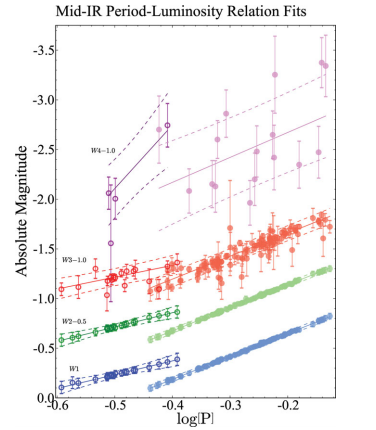
\includegraphics[width=3in]{figures/PL_relation}}
\caption{\it \small{Period-Luminosity relationship of RR Lyrae variable stars. \label{fig:plrelationrrlyrae}}}
  \end{center}
\end{figure}


\subsubsection{Cephedis}

Other variable stars that will be identified are Cephedis Type 1 and Cephedis Type 2.  A typical pulsation period of Cephedis star is $1 - 50$ days Ryden et al. (2010).  These sugergiants span the F, G, and K spectral classes, with average absolute magnitudes between $M=-0.5$ and $M=-6$ Ryden et al. (2010).  The PL relation of Cephedis Type 1 and Cephedis Type 2 is shown in Figure~\ref{fig:cephPL}. From the PL relation we can extract distances Ngeow et al. (2013). Using $m=15$, 30 $s$ exposures will allow for photometric accuracy of 4\%.  A Hertzsprung-Russell diagram of pulsating variable stars is shown by Figure~\ref{fig:var-star-hr} Turner et al. (2012). \textit{Relatively young, star formation epoch?}


%\begin{itemize}
%	\item{} Typical pulsation periods of 1-50 days - need CITATION
	%\item{} F, G, K
	%\item{} Supergiant
	%\item{} Average absolute magnitude -0.5 - -6
	%\item{} All above from B. Ryden and B. Peterson, Foundations of Astrophysics, Pearson, 2010.
	%\item{} Period to Luminosity relations in Ngeow et al. 
	%\item{} From the period to luminosity relations, distance range with $m=15$
%	\item{} Relatively young, star formation epoch?
%\end{itemize}





% side by side figures

\begin{figure}[H]
\centering
\begin{subfigure}{.5\textwidth}
  \centering
  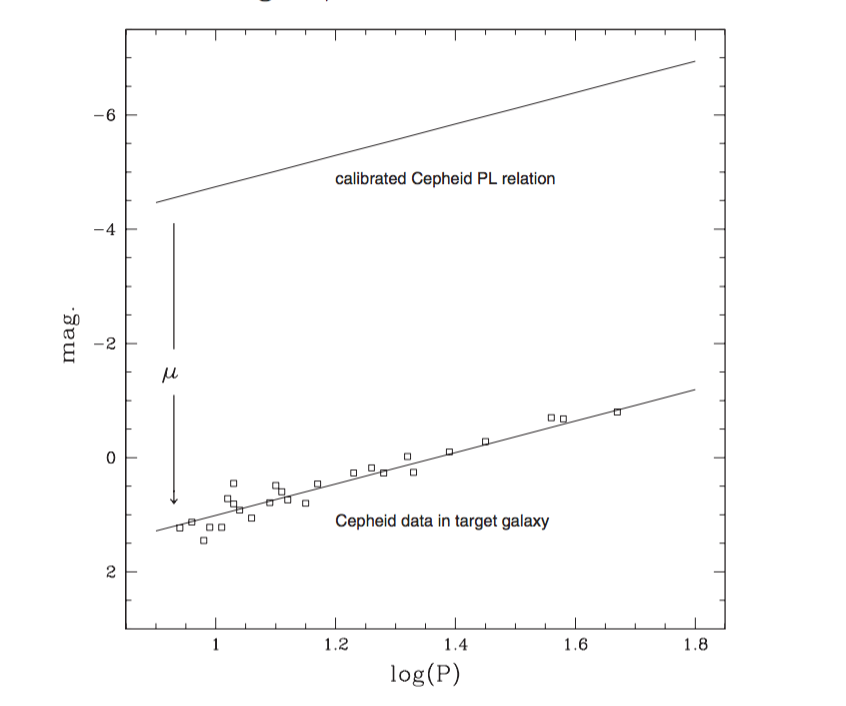
\includegraphics[width=.4\linewidth]{figures/Ngeow1_fig}
  \caption{Period-Luminosity relationship.}
  \label{fig:plrelationrrlyrae}
\end{subfigure}%
\begin{subfigure}{.5\textwidth}
  \centering
  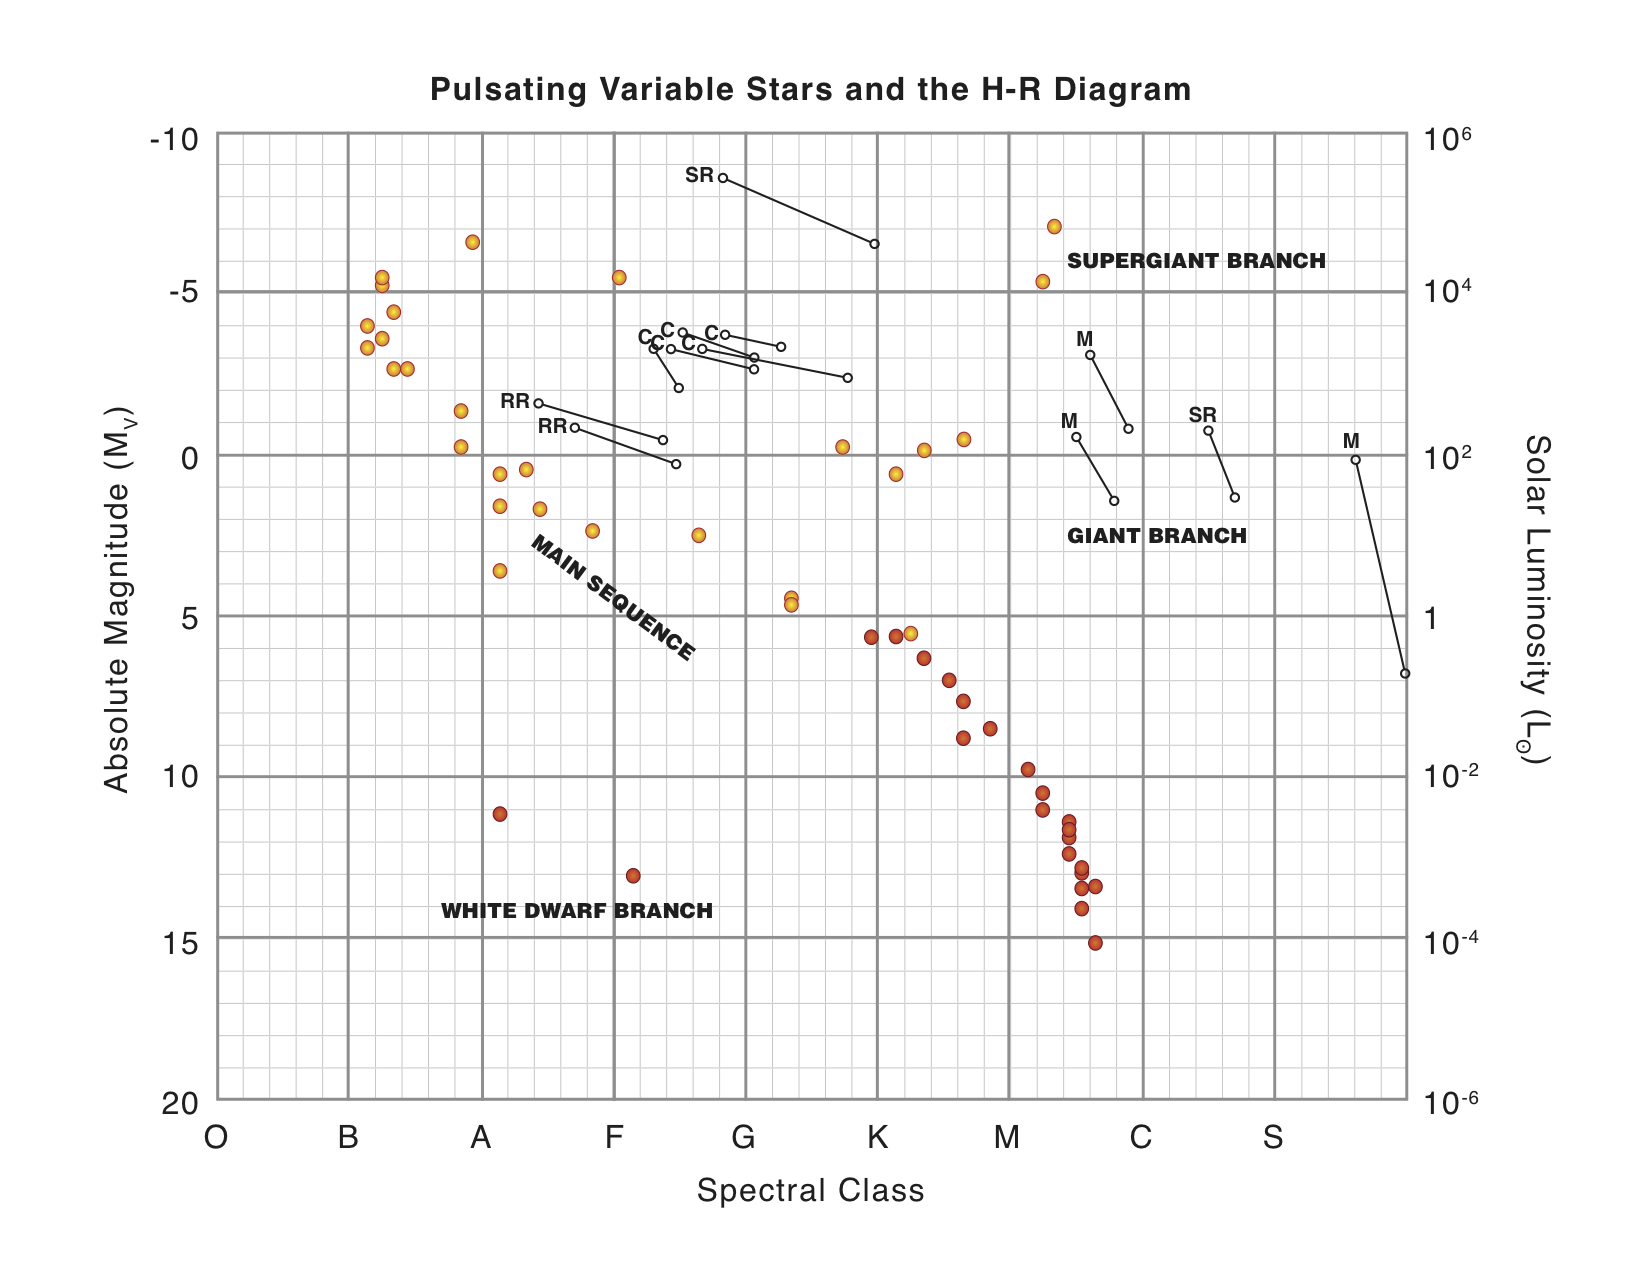
\includegraphics[width=.4\linewidth]{figures/var_star_HR.png}
  \caption{HR-Diagram of pulsating variable stars.}
  \label{fig:var-star-hr}
\end{subfigure}
\caption{Cephedis Type 1 and Cephedis Type 2 stars.}
\label{fig:test}
\end{figure}

\iffalse
\begin{figure}[H]%[htb!]
  \begin{center}
\centerline{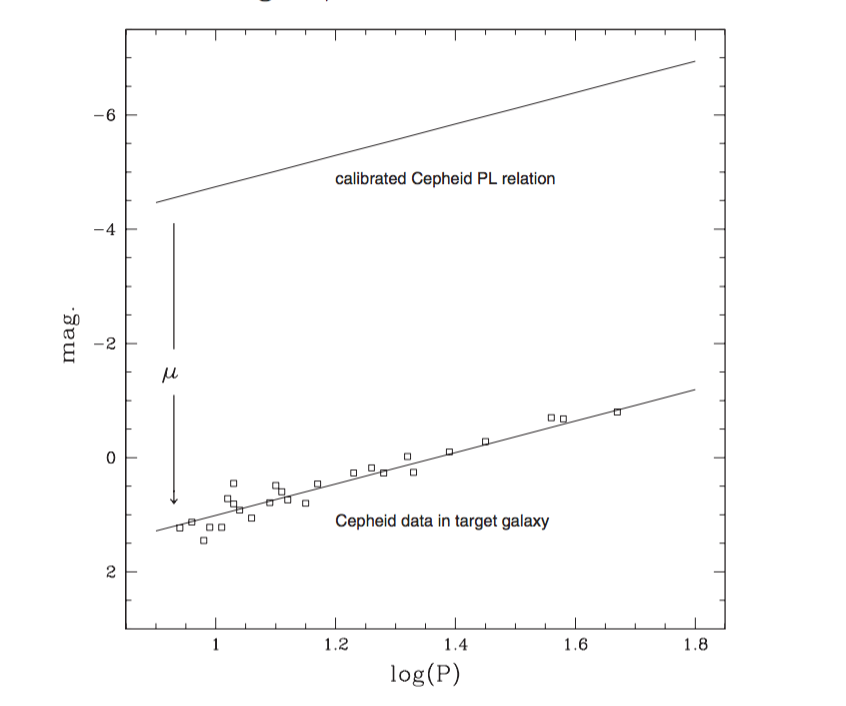
\includegraphics[width=3in]{figures/Ngeow1_fig}}
\caption{\it \small{Period to Luminosity relations of Cephedis stars. \label{fig:cephPL}}}
  \end{center}
\end{figure}

\end{figure}
\begin{figure}[H]%[htb!]
  \begin{center}
\centerline{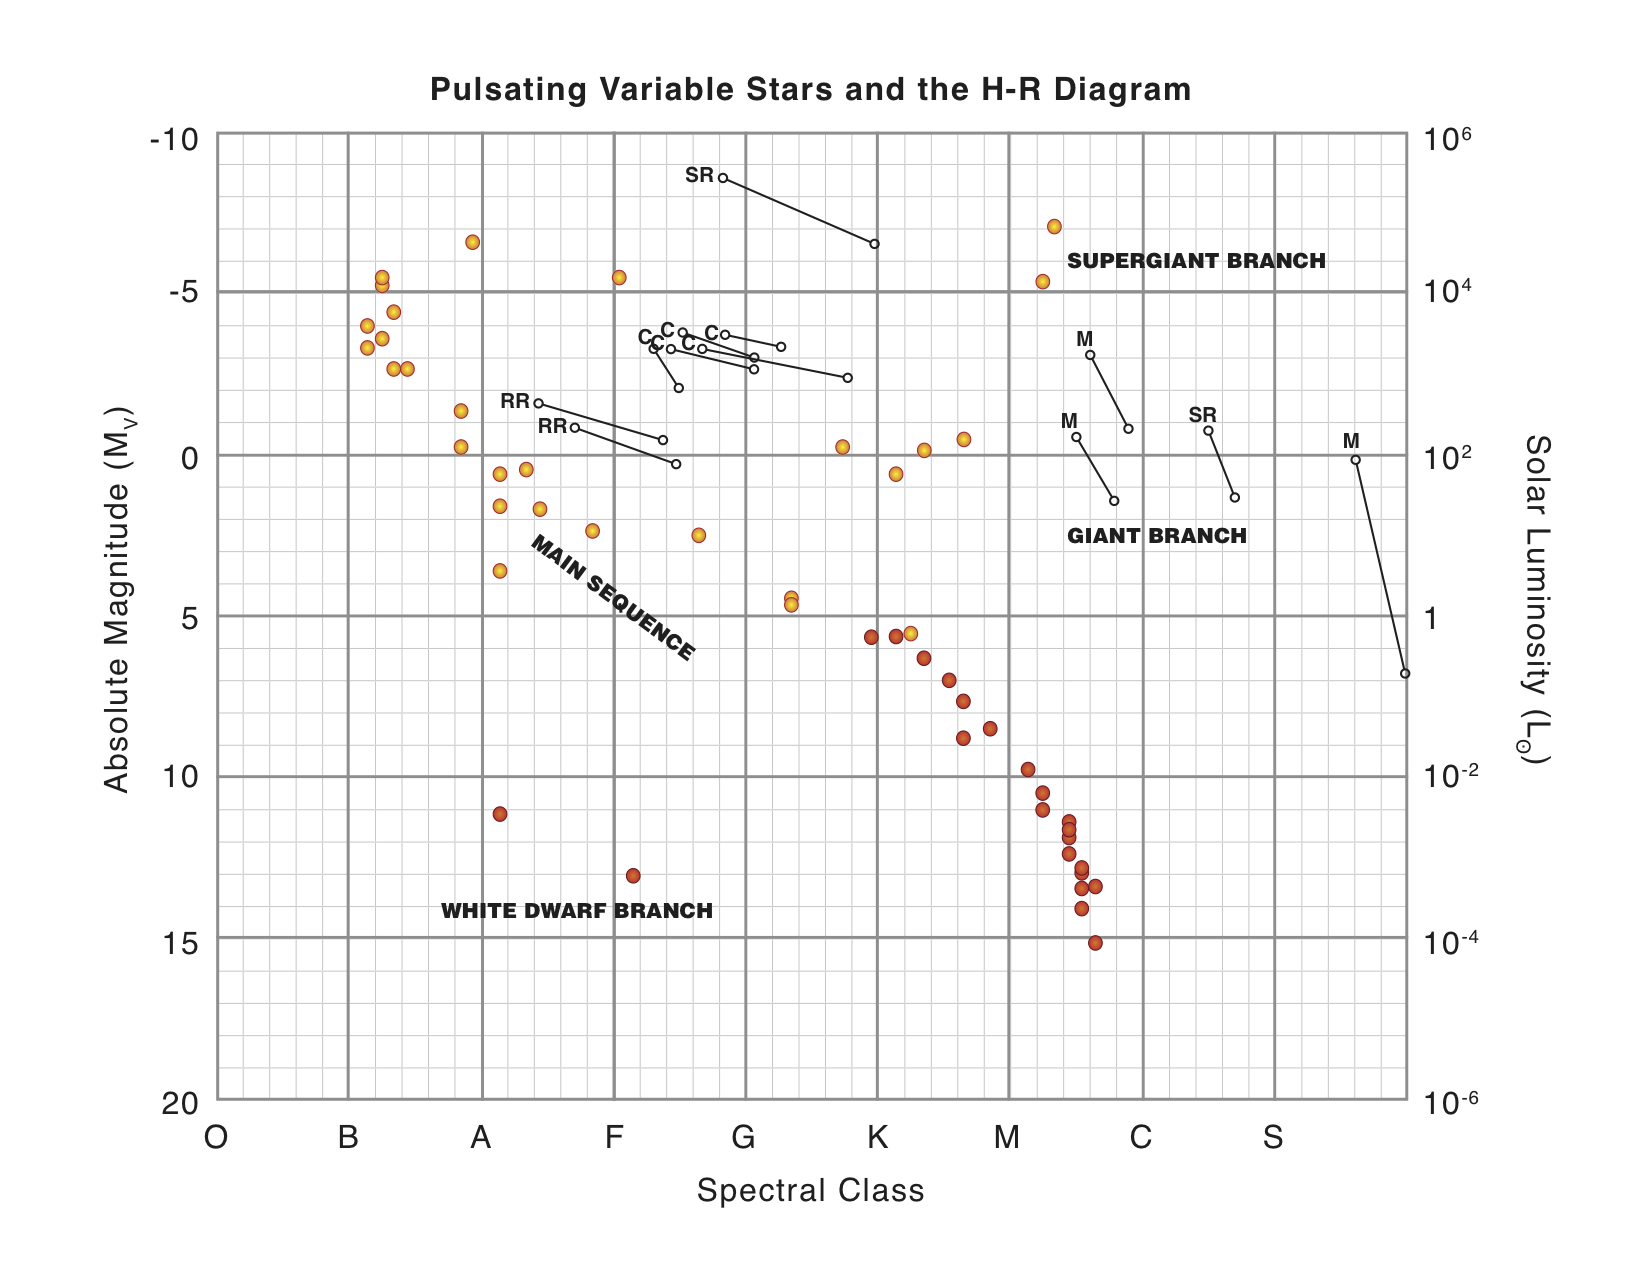
\includegraphics[width=3in]{figures/var_star_HR.png}}
\caption{\it \small{HR-Diagram: Pulsating Variable Stars. \label{fig:var-star-hr}}}
  \end{center}
\end{figure}
\fi

Near the galactic center, ISM is dense, and the number density of stars is high, which makes optical investigations quite difficult. Figure ~ \ref{fig:gas} shows the distribution of gasses in the Milky Way (Nakanishi and Sofue 2015). In order to determine the spiral arm structure of the Milky Way galaxy, we will avoid the galactic center. To take into account for the ISM extinction, we will use the ratio of total to selective extinction $R = \frac{1}{(\tau_{1} / \tau_{2}) -1} = \frac{1}{(\lambda_{eff,1} / \lambda_{eff,2})^{-1} \, -1}$ assuming the optical depth $\tau \propto \lambda^{-1}$ according to the Mie scattering. 

\begin{figure}[H]
  \begin{center}
\centerline{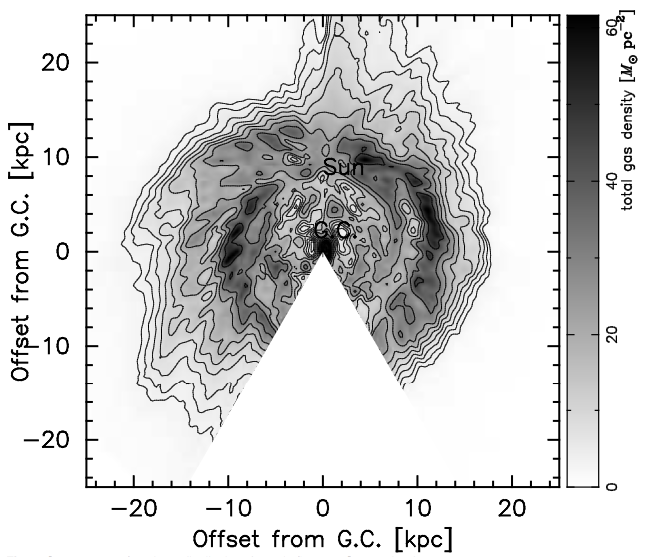
\includegraphics[width=3in]{figures/Gas.png}}
\caption{\it \small{Column density distribution of the sum of HI and H$_2$ gases. \label{fig:gas}}}
  \end{center}
\end{figure}



\section*{References}

\noindent\smallskip{\small
Allen, S.\ et al., 2016. (n.d.). The Classification of Stellar Spectra. Retrieved February 15, 2016, from $http://www.star.ucl.ac.uk/~pac/spectral_classification.html$ \\}

\noindent\smallskip{\small
B.\ et al., 2012. Types of Variables | AAVSO. Retrieved February 16, 2016, from https://www.aavso.org/types-variables \\}

\noindent\smallskip{\small
Nakanishi, H. and Sofue, Y., 2015. Three-Dimensional Distribution of the ISM in the Milky Way Galaxy: III. The Total Neutral Gas Disk. \textit{Publ. Astron. Soc. Japan (2014) 00(0), 1–14}. Retrieved February 15, 2016. \\}

\noindent\smallskip{\small
Ngeow, C.\ et al., 2013. "Distance Determination From The Cepheid And RR Lyrae Period-Luminosity Relations". \textit{Proc. IAU} 9.S301: 123-128. Web. 18 Feb. 2016. \\}


\noindent\smallskip{\small
Ryden, B.\  et al., 2010. Foundations of astrophysics. San Francisco: Addison-Wesley. \\}


\noindent\smallskip{\small
Tsujimoto\ et al., 1998. The Absolute Magnitude of RR Lyrae Stars Derived from the [ITAL]Hipparcos[/ITAL] Catalogue. \textit{The Astrophysical Journal, 492}(1). Retrieved February 15, 2016. \\}

\noindent\smallskip{\small
Turner, R.\ et al., 2012. H-R Diagram Education Materials | AAVSO. Retrieved February 14, 2016, from https://www.aavso.org/hr-diagram-education-materials \\}



\section*{TECHNICAL JUSTIFICATION}


We request $10.3$ hours using Pathfinder to obtain g, r, and i imaging for variable stars in the galactic plane.

\vspace{3mm} %3mm vertical space

\noindent The typical pulsation period of RR Lyrae is in a range of $1.5$ hours to $24$ hours. To sample a $1.5$ hours period, we need to image a RR Lyrae at least twice in one period according to the sampling theorem (\textit{sampling rate vs error?}). With the exposure time of $30$ seconds and readout time of $8$ seconds, the sky coverage rate is $948$ deg$^2$/hour. To cover the galactic plane and avoid the galactic center, we choose a region with galactic latitude of $\pm 2 ^\circ$ and galactic longitude of $70 ^\circ$ to $290 ^\circ$ (\textit{from the gri project, we should be able to choose smaller patches with variable stars on the galactic plane; more points in one period}). The coverage rate and angular size of the field yield the one observation time of $1.14$ hours. We want $3$ band passes with $3$ pulsation periods each to take into account the ISM extinction (\textit{number of periods vs error?}), so we request the total observational time of $10.3$ hours. Since Cepheid stars have longer pulsation periods, we should be able to sample data points well.

\vspace{3mm} %3mm vertical space

\noindent The SNRs of g, r, and i bands with $m_g = m_r = m_i = 15$ are $26.11$, $26.31$, and $20.67$, respectively. We use relative intensity to measure pulsation periods, so this photometric accuracy of $4 \%$ should be enough (\textit{photometric accuracy vs error?}).


\section*{Things to Discuss Further}

\begin{itemize}
	%\item{} Use gri data to identify variable Stars 		
	%\item{} Use Period-Luminosity relationship to get distance 
	%\item{} Map 3D spatial distribution
	%\item{} Distance Equation
	\item{} Determine deviation of variable stars from model
	\item{} Variations arise from gravitational effects from unknown sources
	\item{} Figure out dark matter distribution
	\item{} include - Plot of known var star distributions in spiral arms
	\item{} comment on knowing m from tying into pan-starrs
	\item{} difference in 3 variable stars light curves - show examples
\end{itemize}


\end{document}